\scanpage{36}

\margin{\unsure{15|25}.11.66}

Nous avons montré que la cohomologie \deleted{de D.R.} \inserted{complexe ordinaire} d'une variété algébrique non singulière sur $\mathbb C$ \unsure{se décrit} par voie purement algébrique comme ``cohomologie de De Rham''
\[
H_{\mathrm{DR}}(X)=\mathbb H^*(X;\Omega_X^\bullet)
\]
\margin{\figure{\begin{tikzpicture}\draw (0,0)--(.24,.06);\end{tikzpicture}}}

Celle-ci a un sens pour n'importe quel schéma sur un corps quelconque. Cependant cette version de la cohomologie \unsure{nombreux} désavantages : liée aux formes diff donc aux variétés non sing, \inserted{le corps de \deleted{coefficient} base de la théorie coh. \unsure{peut} être de car $p>0$\ldots}

D'autre part, nous avons vu la désirabilité d'avoir une théorie de cohomologie ``$p$-adique'' pour les variétés en car. $p$, pour jouer le $\overline{\mathrm m}$ rôle que les \unsure{cohomologies} $\ell$-adiques, $\ell\ne p$. On veut les $\overline{\mathrm m}\mathrm s$ nbs de Betti etc \ldots

Une remarque sur la définition de la coh. de De Rham : $\underline{\Omega}^1_{X/S}$ est défini pour tt préschéma relatif $X/S$, et $\bigwedge^*\underline{\Omega}^1_{X/S}=\underline{\Omega}^*_{X/S}$ est muni d'un op. diff naturel\ldots\ On peut donc définir
\[
\left\{
\begin{aligned}
&H_{\mathrm{DR}}(X/S)=\mathbb H^*(X,\underline{\Omega}^*_{X/S})\\
&\text{et les }\mathbb R f_*(\underline{\Omega}^\bullet_{X/S})
\end{aligned}
\right.
\]

\margin{\figure{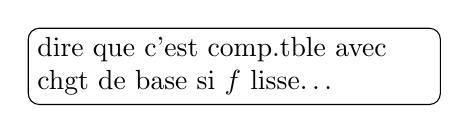
\begin{tikzpicture}
\node[draw,rounded corners,align=left,text width=5cm] at (0,0) {dire que c'est \unsure{comp.tble} avec chgt de base \unsure{si} $f$ \uline{lisse}\ldots};
\end{tikzpicture}}}

\margin{(coh. si $\left\{\begin{array}{l}
f\ \text{propre et }\unsure{\text{lisse}}\\
\text{ou }f\ \text{propre}, S\ \text{loc }\unsure{\text{noeth}}
\end{array}\right.$}

\margin{35}
